\documentclass[a4paper, 12pt]{article}

\input{/home/nick/latex-preambles/xelatex.tex}

\setmainfont{Minion Pro}

\newcommand{\imagesPath}{.}

\title{
	\textbf{Εργαστήριο Δικτύων Υπολογιστών} \\~\\
	Εργαστηριακή Άσκηση 11 \\ 
	Το πρωτόκολλο IPv6
}
\author{}
\date{}

\begin{document}
\maketitle
\begin{center}
	\begin{tabular}{|l|l|}
		\hline
		\textbf{Ονοματεπώνυμο:} Νικόλαος Παγώνας, el18175  & \textbf{Όνομα PC:} nick-ubuntu \\
		\hline
		\textbf{Ομάδα:} 1 (Τρίτη 10:45) & \textbf{Ημερομηνία Εξέτασης:} Τρίτη 24/05/2022 \\
		\hline
	\end{tabular}
\end{center}

\section*{Άσκηση 1: Εισαγωγή στο IPv6}

	\subsection*{Προετοιμασία στο σπίτι}

		\subsubsection*{1.}
			Εκτελούμε \verb|service frr stop|.

		\subsubsection*{2.}
			Εκτελούμε \verb|touch /usr/local/etc/frr/ripngd.conf|.

		\subsubsection*{3.}
			Εκτελούμε \verb|touch /usr/local/etc/frr/ospf6d.conf|.

		\subsubsection*{4.}
			Εκτελούμε \verb|chown frr:frr /usr/local/etc/frr/{ripngd.conf,ospf6d.conf}|
		
		\subsubsection*{5.}
			Αλλάζουμε τη ζητούμενη γραμμή σε:
			
			\begin{verbatim}
				frr_daemons="zebra staticd ripd ripngd ospfd ospf6d bgpd"
			\end{verbatim}

		\subsubsection*{6.}
			Εκτελούμε:
			
			\begin{verbatim}
				reboot
				service sshd status
				service frr status
			\end{verbatim}
			
			Τρέχουν κανονικά.

		\subsubsection*{7.}
			Εκτελούμε \verb|service frr start|.

		\subsubsection*{8.}
			Εκτελούμε: 
			
			\begin{verbatim}
				poweroff
				File - Export Appliance...
			\end{verbatim}
			
			και δημιουργούμε ένα αρχείο \verb|frr.ova|.

		\subsubsection*{9.}
			Αποθηκεύουμε το \verb|frr.ova| για μελλοντική χρήση.
		
	\subsection*{1.1}
		Εκτελούμε:
		
		\begin{verbatim}
			### PC1 ###
			
			sysrc ifconfig_em0_ipv6="inet6 accept_rtadv" 
			
			### PC2 ###

			sysrc ifconfig_em0_ipv6="inet6 accept_rtadv" 
		\end{verbatim}

	\subsection*{1.2}
		Εκτελούμε:
		
		\begin{verbatim}
			### PC1 ###
			
			service netif restart
			
			### PC2 ###
			
			service netif restart
		\end{verbatim}

	\subsection*{1.3}
		Στο PC1 εκτελούμε \verb|ifconfig em0|. Έχει αποδοθεί η διεύθυνση \verb|fe80::a00:27ff:fe96:db|.

	\subsection*{1.4}
		Στο PC2 εκτελούμε \verb|ifconfig em0|. Έχει αποδοθεί η διεύθυνση \verb|fe80::a00:27ff:fe25:d99f|.

	\subsection*{1.5}
		Είναι είδους link-local (\verb|fe80::/10|). Προκύπτει ως εξής:
		
		\begin{verbatim}
			### PC1 ###
						
			08 00 27 96 00 db                                   (MAC address)
			
			08 00 27 ff fe 96 00 db                             (ff fe in the middle)
			
			0a 00 27 ff fe 96 00 db                             (Flip 7th bit of 1st byte)
			
			fe 80 00 00 00 00 00 00 0a 00 27 ff fe 96 00 db     (Insert fe80::/10 prefix)
			
			fe80:0000:0000:0000:0a00:27ff:fe96:00db             (IP address with leading 0s)
			
			fe80::a00:27ff:fe96:db                              (Final IP address)
			
			### PC2 ###
						
			08 00 27 25 d9 9f                                   (MAC address)
			
			08 00 27 ff fe 25 d9 9f                             (ff fe in the middle)
			
			0a 00 27 ff fe 25 d9 9f                             (Flip 7th bit of 1st byte)
			
			fe 80 00 00 00 00 00 00 0a 00 27 ff fe 25 d9 9f     (Insert fe80::/10 prefix)
			
			fe80:0000:0000:0000:0a00:27ff:fe25:d99f             (IP address with leading 0s)
			
			fe80::a00:27ff:fe25:d99f                            (Final IP address)
		\end{verbatim}

	\subsection*{1.6}
		Στο PC1 εκτελούμε \verb|netstat -rn6|. Εμφανίζονται 9 εγγραφές:
		
		\begin{verbatim}
			Destination                      Gateway       Flags       Netif 
			::/96                            ::1           UGRS        lo0
			::1                              link#2        UH          lo0
			::ffff:0.0.0.0/96                ::1           UGRS        lo0
			fe80::/10                        ::1           UGRS        lo0
			fe80::%em0/64                    link#1        U           em0
			fe80::a00:27ff:fe96:db%em0       link#1        UHS         lo0
			fe80::%lo0/64                    link#2        U           lo0
			fe80::1%lo0                      link#2        UHS         lo0
			ff02::/16                        ::1           UGRS        lo0
		\end{verbatim}

	\subsection*{1.7}
		Μία εγγραφή αφορά την \verb|em0|:
		
		\begin{verbatim}
			Destination         Gateway       Flags       Netif
			fe80::%em0/64       link#1        U           em0
		\end{verbatim}

	\subsection*{1.8}
		Περιέχει τις εγγραφές:
		
		\begin{verbatim}
			Destination                      Gateway       Flags       Netif
			fe80::%em0/64                    link#1        U           em0
			fe80::a00:27ff:fe96:db%em0       link#1        UHS         lo0
			fe80::%lo0/64                    link#2        U           lo0
			fe80::1%lo0                      link#2        UHS         lo0
		\end{verbatim}

	\subsection*{1.9}
		Στο PC1 εκτελούμε \verb|ping6 ::1|. Απαντά το ίδιο το PC1.
	
	\subsection*{1.10}
		Στο PC1 εκτελούμε \verb|ping6 fe80::a00:27ff:fe96:db|. Εμφανίζεται μήνυμα λάθους "UDP connect: Network is unreachable". Πρέπει να προσθέσουμε τον δείκτη ζώνης \verb|%em0| στο τέλος της διεύθυνσης ως εξής:
		
		\begin{verbatim}
			ping6 fe80::a00:27ff:fe96:db%em0
		\end{verbatim}
		
		Τώρα το ping είναι επιτυχές.
	
	\subsection*{1.11}
		Στο PC1 εκτελούμε \verb|ping6 fe80::a00:27ff:fe25:d99f|. Αποτυγχάνει όπως και πριν με μήνυμα λάθους "UDP connect: Network is unreachable". Προσθέτουμε τον δείκτη ζώνης \verb|%em0|:
		
		\begin{verbatim}
			ping6 fe80::a00:27ff:fe25:d99f%em0
		\end{verbatim}
		
		Το ping είναι επιτυχές.
	
	\subsection*{1.12}
		Στο PC1 εκτελούμε \verb|ping6 -I em0 ff01::1|. Απαντά το PC1, αφού η διεύθυνση \verb|ff01::1| παριστάνει όλους τους κόμβους στη διεπαφή.

	\subsection*{1.13}
		Στο PC1 εκτελούμε \verb|ping6 -I em0 ff02::1|. Απαντούν τα PC1 και PC2, αφού η διεύθυνση \verb|ff02::1| παριστάνει όλους τους κόμβους στην τοπική ζεύξη.

	\subsection*{1.14}
		Στο PC1 εκτελούμε \verb|ifconfig em0 inet6 fd00:1::2/64|.

	\subsection*{1.15}
		Στο PC2 εκτελούμε \verb|ifconfig em0 inet6 fd00:1::3/64|.

	\subsection*{1.16}
		Είναι μοναδικές τοπικές διευθύνσεις (\verb|fd00::/8|), οι ανάλογες των διευθύνσεων ιδιωτικής χρήσης \verb|10.0.0.0/8, 172.16.0.0/12, 192.168.0.0/16| στο IPv4.
		
	\subsection*{1.17}
		Στα PC1 και PC2 εκτελούμε \verb|ifconfig em0|. Υπάρχουν 2 διευθύνσεις. 

	\subsection*{1.18}
		Στο PC1 εκτελούμε \verb|netstat -rn6|. Προστέθηκαν 2 νέες εγγραφές (επισημαίνονται με \verb|+++| στην αρχή της γραμμής):
		
		\begin{verbatim}
			    Destination                    Gateway      Flags      Netif
			    ::/96                          ::1          UGRS       lo0 
			    ::1                            link#2       UH         lo0
			    ::ffff:0.0.0.0/96              ::1          UGRS       lo0
			+++ fd00:1::/64                    link#1       U          em0
			+++ fd00:1::2                      link#1       UHS        lo0
			    fe80::/10                      ::1          UGRS       lo0
			    fe80::%em0/64                  link#1       U          em0
			    fe80::a00:27ff:fe96:db%em0     link#1       UHS        lo0
			    fe80::%lo0/64                  link#2       U          lo0
			    fe80:1%lo0                     link#2       UHS        lo0
			    ff02::/16                      ::1          UGRS       lo0
		\end{verbatim}

	\subsection*{1.19}
		Πρέπει και στα δύο μηχανήματα να προσθέσουμε (μέσω \verb|vi /etc/hosts|) τις γραμμές:
		
		\begin{verbatim}
			fd00:1::2 PC1
			fd00:1::3 PC2
		\end{verbatim}

	\subsection*{1.20}
		Στο PC1 εκτελούμε \verb|ping6 PC2|. Το ping είναι επιτυχές.

	\subsection*{1.21}
		Στο PC1 εκτελούμε \verb|arp -a|. Δεν παρατηρούμε καμία εγγραφή.

	\subsection*{1.22}
		Στο PC1 εκτελούμε \verb|man ndp|.

	\subsection*{1.23}
		Είναι \verb|npd -a|.

	\subsection*{1.24}
		Βλέπουμε 4 εγγραφές:
		
		\begin{verbatim}
			Neighbor                      Linklayer Addr     Netif  Expire     S  Flags
			PC1                           08:00:27:96:00:db  em0    permanent  R
			PC2                           08:00:27:25:d9:9f  em0    23h58m7s   S
			fe80::a00:27ff:fe96:db%em0    08:00:27:96:00:db  em0    permanent  R
			fe80::a00:27ff:fe25:d99f%em0  08:00:27:25:d9:9f  em0    22h7m44s   S
		\end{verbatim}

	\subsection*{1.25}
		Στο PC1 εκτελούμε \verb|ndp -p|. Έχουμε:
		
		\begin{verbatim}
			fd00:1::/64 if=em0
			flags=LO vltime=infinity, pltime=infinity, expire=Never, ref=1
			  No advertising router
			
			fe80::%em0/64 if=em0
			flags=LAO vltime=infinity, pltime=infinity, expire=Never, ref=0
			  No advertising router
			
			fe80::%lo0/64 if=lo0
			flags=LAO vltime=infinity, pltime=infinity, expire=Never, ref=0
			  No advertising router
		\end{verbatim}
		
		Οι εγγραφές έχουν άπειρη διάρκεια ζωής. Από το SLAAC μπορούν να χρησιμοποιηθούν η 2η και η 3η εγγραφή, που έχουν τη σημαία "A" ενεργοποιημένη.

	\subsection*{1.26}
		Σε νέο παράθυρο στο PC2 εκτελούμε \verb|tcpdump -vn|.

	\subsection*{1.27}
		Στα PC1 και PC2 εκτελούμε \verb|ndp -c|.

	\subsection*{1.28}
		Στο PC1 εκτελούμε \verb|ping6 -c 1 PC2| και σταματάμε την καταγραφή. Βλέπουμε 6 πακέτα IPv6.

	\subsection*{1.29}
		Μεταφέρουν μηνύματα του ICMPv6. Η τιμή του Next header είναι 58.

	\subsection*{1.30}
		\begin{figure}[H]
			\begin{center}
				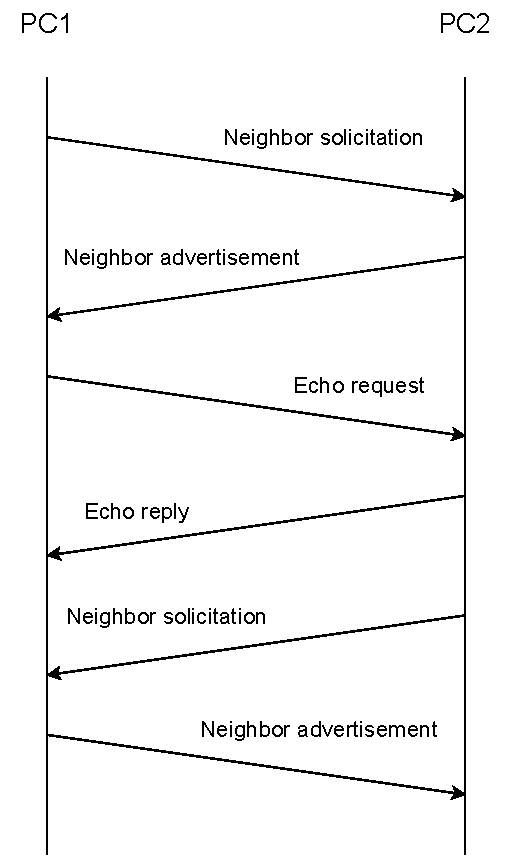
\includegraphics[width=0.5\linewidth]{\imagesPath/1.30.pdf}
			\end{center}
		\end{figure}

	\subsection*{1.31}
		Η διεύθυνση προορισμού του πρώτου πακέτου NS (\verb|ff02::1:ff00:3|) είναι multicast Solicited Node και προκύπτει από τα τελευταία 24 bit της διεύθυνσης unicast του PC2, αν σε αυτά προσθέσουμε το πρόθεμα \verb|ff02:0:0:0:0:1:ff00:0/104|:
		
		\begin{verbatim}
		    ff02:0:0:0:0:1:ff00:0000    (Special prefix)
		+                    00:0003    (Last 24 bits of PC2 unicast address)
		----------------------------
		    ff02:0:0:0:0:1:ff00:0003    (Multicast Solicited Node address with leading 0s)
		    
		              ff02::1:ff00:3    (Final multicast Solicited Node address)
		\end{verbatim}

	\subsection*{1.32}
		Η διεύθυνση προορισμού του δεύτερου πακέτου NS (\verb|fd00:1::2|) είναι μοναδική τοπική διεύθυνση, και έχει προκύψει από ανάθεση (που έγινε σε προηγούμενο ερώτημα).

	\subsection*{1.33}
		Στο PC2 εκτελούμε \verb|ndp -a|. Η κατάσταση της εγγραφής για το PC1 είναι "S" (Stale). Η διάρκεια ζωής της σχετικής εγγραφής είναι \verb|22h1m44s|.

	\subsection*{1.34}
		Στο PC1 εκτελούμε \verb|ping6 PC2| και ύστερα με διαδοχικά \verb|ndp -a| στο PC2 παρατηρούμε συνεχή εναλλαγή μεταξύ των καταστάσεων "R" και "S" (Reachable και Stale).

	\subsection*{1.35}
		Φαίνεται να είναι $\approx$43 δευτερόλεπτα, και μόλις λήξει, η αντίστοιχη εγγραφή μπαίνει σε κατάσταση Stale.

	\subsection*{1.36}
		Είναι 24 ώρες.

	\subsection*{1.37}
		Σταματάμε το ping στο PC1 και ύστερα με διαδοχικά \verb|ndp -a| στο PC2 παρατηρούμε αλλαγή από την κατάσταση "R" (Reachable) στην κατάσταση "S" (Stale), και αυτή τη φορά η κατάσταση παραμένει "S" (Stale).

	\subsection*{1.38}
		Στο PC1 εκτελούμε \verb|ping6 PC2|. Στο PC2 εκτελούμε \verb|tcpdump -n|. Παρατηρούμε επιπλέον πακέτα ICMPv6 neighbor solicitation (NS), με σκοπό να επιβεβαιωθεί η προσβασιμότητα του γείτονα, και ICMPv6 neighbor advertisement (NA), ως απάντηση στα πακέτα NS. Παράγονται περίπου κάθε 23 δευτερόλεπτα.

\section*{Άσκηση 2: SLAAC και Στατική δρομολόγηση IPv6}

	\subsection*{2.1}
		Στους R1 και R2 εκτελούμε:
		
		\begin{verbatim}
			sysrc ipv6_gateway_enable="YES"
			service routing restart
		\end{verbatim} 

	\subsection*{2.2}
		Στο PC2 εκτελούμε:
		
		\begin{verbatim}
			ifconfig em0 inet6 fd00:1::3/64 delete
			ifconfig em0 inet6 fd00:2::2/64
		\end{verbatim}

	\subsection*{2.3}
		Στον R1 εκτελούμε:
		
		\begin{verbatim}
			vtysh
			configure terminal
			
			interface em0
			
			ipv6 address fd00:1::1/64 
		\end{verbatim}
		
		\textbf{Σημείωση:} Μπορούμε να δώσουμε και την εντολή \verb|"ip address"| αντί για \verb|"ipv6 address"|. Και στις δύο περιπτώσεις η εντολή θα καταχωρηθεί ως \verb|"ipv6 address"| στο running configuration. Εμείς προτιμούμε την εντολή \verb|"ipv6 address"| για να είμαστε απολύτως ακριβείς.

	\subsection*{2.4}
		Στον R1 εκτελούμε:
		
		\begin{verbatim}
			interface em1
			ipv6 address fd00:3::1/126
		\end{verbatim}

	\subsection*{2.5}
		Στον R2 εκτελούμε:
		
		\begin{verbatim}
			vtysh
			configure terminal
			
			interface em1
			ipv6 address fd00:2::1/64
		\end{verbatim}

	\subsection*{2.6}
		Στον R2 εκτελούμε:
		
		\begin{verbatim}
			interface em0
			ipv6 address fd00:3::2/126
		\end{verbatim}

	\subsection*{2.7}
		Στο PC1 εκτελούμε \verb|route -6 add default fd00:1::1|.

	\subsection*{2.8}
		Στο PC2 εκτελούμε \verb|route -6 add default fd00:2::1|.

	\subsection*{2.9}
		Στον R1 εκτελούμε \verb|tcpdump -i em0|. 

	\subsection*{2.10}
		Στο PC1 εκτελούμε:
		
		\begin{verbatim}
			ndp -c
			ping6 -c 1 fd00:2::2
		\end{verbatim}
		
		Δε λαμβάνουμε απάντηση. Αυτό συμβαίνει διότι ο R1 δεν διαθέτει εγγραφή στον πίνακα δρομολόγησης σχετική με τη διεύθυνση \verb|fd00:2::2| και έτσι στέλνει μήνυμα λάθους ICMPv6 destination unreachable.

	\subsection*{2.11}
		Παράγονται (καταγράφουμε και την διεύθυνση πηγής για πληρότητα):
		
		\begin{verbatim}
			ICMPv6 Message                IPv6 source address       IPv6 destination address 
			Neighbor solicitation         fd00:1::2                 ff02::1:ff00:1 
			Neighbor advertisement        fd00:1::1                 fd00:1::2
			Echo request                  fd00:1::2                 fd00:2::2
			Destination unreachable       fd00:1::1                 fd00:1::2
			Neighbor solicitation         fd00:1::1                 fd00:1::2
			Neighbor advertisement        fd00:1::2                 fd00:1::1
		\end{verbatim}

	\subsection*{2.12}
		Στον R1 εκτελούμε:
		
		\begin{verbatim}
			ipv6 route fd00:2::/64 fd00:3::2
		\end{verbatim}
		
		\textbf{Σημείωση:} Όπως και πριν, επιλέγουμε την εντολή \verb|"ipv6"|, αλλά και η \verb|"ip"| θα είχε τα ίδια αποτελέσματα (στο running configuration η εντολή καταχωρείται έτσι κι αλλιώς ως \verb|"ipv6"|).

	\subsection*{2.13}
		Στο PC1 εκτελούμε \verb|ping6 -c 1 fd00:2::2|. Δεν λαμβάνουμε απάντηση, διότι ο R2 δεν έχει εγγραφή στον πίνακα δρομολόγησης σχετική με τη διεύθυνση \verb|fd00:1::2| προκειμένου να στείλει το ICMPv6 echo reply.

	\subsection*{2.14}
		Στον R2 εκτελούμε:
		
		\begin{verbatim}
			ipv6 route fd00:1::/64 fd00:3::1 
		\end{verbatim} 

	\subsection*{2.15}
		Στο PC1 εκτελούμε \verb|ping6 -c 1 fd00:2::2|. Το ping είναι επιτυχές.

	\subsection*{2.16}
		Στον R1 εκτελούμε:
		
		\begin{verbatim}
			interface em0
			no ipv6 nd suppress-ra
		\end{verbatim}

	\subsection*{2.17}
		Στον R1 εκτελούμε:
		
		\begin{verbatim}
			interface em0
			ipv6 nd prefix fd00:1::/64
		\end{verbatim}

	\subsection*{2.18}
		Στον R2 εκτελούμε:
		
		\begin{verbatim}
			interface em1
			no ipv6 nd suppress-ra
		\end{verbatim}

	\subsection*{2.19}
		Στον R2 εκτελούμε:
		
		\begin{verbatim}
			interface em1
			ipv6 nd prefix fd00:2::/64
		\end{verbatim}

	\subsection*{2.20}
		Στο PC1 εκτελούμε:
		
		\begin{verbatim}
			route -6 delete default 
		\end{verbatim}

	\subsection*{2.21}
		Στον R1 εκτελούμε \verb|tcpdump -eni em0 icmp6|.

	\subsection*{2.22}
		Στο PC1 εκτελούμε \verb|service netif restart|.

	\subsection*{2.23}
		Ανταλλάσονται τα μηνύματα: \\
		
		\begin{tabular}{|l|l|l|l|l|}
			\hline
			\textbf{Type} &    \textbf{MAC source}     &  \textbf{MAC destination}  &       \textbf{IPv6 source}        & \textbf{IPv6 destination} \\ 
			\hline
			 NS  & 08:00:27:96:00:DB & 33:33:FF:96:00:DB &            ::            & FF02::1:FF96:DB  \\
			 \hline
			 RS  & 08:00:27:96:00:DB & 33:33:00:00:00:02 &  FE80::A00:27FF:FE96:DB  &     FF02::2      \\
			 \hline
			 RA  & 08:00:27:03:C1:F6 & 33:33:00:00:00:01 & FE80::A00:27FF:FE03:C1F6 &     FF02::1      \\
			 \hline
			 NS  & 08:00:27:96:00:DB & 33:33:FF:96:00:DB &            ::            & FF02::1:FF96:DB  \\ 
			 \hline
		\end{tabular}

	\subsection*{2.24}
		Παράγει 2 μηνύματα NS. Το πρώτο από αυτά χρειάζεται για την αυτόματη απόδοση διεύθυνσης και το δεύτερο για την ανίχνευση ταυτόσημων διευθύνσεων.

	\subsection*{2.25}
		Χρησιμοποιεί την \verb|::| (Μη ορισμένη/Unspecified) και στα δύο, στο πρώτο NS επειδή ο PC1 δεν έχει αποκτήσει ακόμα διεύθυνση, και στο δεύτερο NS επειδή κατά τη διαδικασία DAD χρησιμοποιείται πάντα η ακαθόριστη διεύθυνση \verb|::|.

	\subsection*{2.26}
		Χρησιμοποιεί την \verb|fe80::a00:27ff:fe96:db|.

	\subsection*{2.27} 
		Είναι:
		
		\begin{verbatim}
			Type     IPv6 destination address
			NS       ff02::1:ff96:db
			RS       ff02::2
			RA       ff02::1
			NS       ff02::1:ff96:db
		\end{verbatim}

		\begin{itemize}
			\item Το NS έχει αυτή τη διεύθυνση επειδή αναφέρεται στην τοπική ζεύξη $\rightarrow$ στον PC1
			\item Το RS έχει αυτή τη διεύθυνση επειδή αναφέρεται σε όλους τους δρομολογητές στην τοπική ζεύξη.
			\item Το RA έχει αυτή τη διεύθυνση επειδή αναφέρεται σε όλους τους κόμβους της τοπικής ζεύξης.
			\item Τέλος, το δεύτερο NS έχει διεύθυνση ίδια με το παραπάνω NS.
		\end{itemize}

	\subsection*{2.28}
		Είναι:
		
		\begin{verbatim}
			Type      MAC destination address
			NS        33:33:ff:96:00:db
			RS        33:33:00:00:00:02
			RA        33:33:00:00:00:01
			NS        33:33:ff:96:00:db
		\end{verbatim}
		
		Οι παραπάνω διευθύνσεις MAC προορισμού προκύπτουν από την παράθεση του προθέματος \verb|33:33:| να ακολουθείται από τα τελευταία 32 bit της IPv6 διεύθυνσης προορισμού, επομένως:
		
		\begin{verbatim} 
			### NS ###
			ff 02 00 00 00 00 00 00 00 00 00 01 ff 96 00 db    (IPv6 destination address)
			                                    ff 96 00 db    (Last 32 bits)
			                              33 33 ff 96 00 db    (Add 33 33 prefix)			
			                              33:33:ff:96:00:db    (Final MAC address)
		\end{verbatim}
		
		\begin{verbatim} 
			### RS ###
			ff 02 00 00 00 00 00 00 00 00 00 00 00 00 00 02    (IPv6 destination address)
			                                    00 00 00 02    (Last 32 bits)
			                              33 33 00 00 00 02    (Add 33 33 prefix)
			                              33:33:00:00:00:02    (Final MAC address)
		\end{verbatim}
	
		\begin{verbatim} 
	
			### RA ###
			ff 02 00 00 00 00 00 00 00 00 00 00 00 00 00 01    (IPv6 destination address)
			                                    00 00 00 01    (Last 32 bits)
			                              33 33 00 00 00 01    (Add 33 33 prefix)
			                              33:33:00:00:00:01    (Final MAC address)
	
		\end{verbatim}
		
		\begin{verbatim} 
			### NS ###
			ff 02 00 00 00 00 00 00 00 00 00 01 ff 96 00 db    (IPv6 destination address)
			                                    ff 96 00 db    (Last 32 bits)
			                              33 33 ff 96 00 db    (Add 33 33 prefix)
			                              33:33:ff:96:00:db    (Final MAC address)	
		\end{verbatim}

	\subsection*{2.29}
		Στο PC1 εκτελούμε \verb|ndp -p|. Έχουμε:
		
		\begin{verbatim}
			fd00:1::/64 if=em0
			flags=LAO vltime=2592000, pltime=604800, expire=29d23h51m54s, ref=1
			  advertised by
			    fe80::a00:27ff:fe03:c1f6%em0 (reachable)
			
			fe80::%em0/64 if=em0
			flags=LAO vltime=infinity, pltime=infinity, expire=Never, ref=0
			  No advertising router
			
			fe80::%lo0/64 if=lo0
			flags=LAO vltime=infinity, pltime=infinity, expire=Never, ref=0
			  No advertising router
		\end{verbatim}
		
		Πλέον έχει μαθευτεί το πρόθεμα \verb|fd00:1::/64| που διαφημίζει ο R1 (\verb|fe80::a00:27ff:fe03:c1f6|).

	\subsection*{2.30}
		Στο PC1 εκτελούμε \verb|ifconfig em0|. Το PC1 έχει λάβει αυτόματα μέσω του SLAAC τη διεύθυνση \verb|fd00:1::a00:27ff:fe96:db|. 

	\subsection*{2.31}
		Στο PC1 εκτελούμε \verb|netstat -rn6|. Έχουμε:
		
		\begin{verbatim}
			Destination                 Gateway                       Flags  Netif
			::/96                       ::1                           UGRS   lo0
			default                     fe80::a00:27ff:fe03:c1f6%em0  UG     em0
			::1                         link#2                        UH     lo0
			::ffff:0.0.0.0/96           ::1                           UGRS   lo0
			fd00:1::/64                 link#1                        U      em0
			fd00:1::a00:27ff:fe96:db    link#1                        UHS    lo0
			fe80::/10                   ::1                           UGRS   lo0
			fe80::%em0/64               link#1                        U      em0
			fe80::a00:27ff:fe96:db%em0  link#1                        UHS    lo0
			fe80::%lo0/64               link#2                        U      lo0
			fe80::1%lo0                 link#2                        UHS    lo0
			ff02::/16                   ::1                           UGRS   lo0
		\end{verbatim}
		
		Υπάρχει προκαθορισμένη διαδρομή (είναι η δεύτερη εγγραφή στον παραπάνω πίνακα). Προέκυψε από τα μηνύματα Router advertisement που έστειλε ο R1.

	\subsection*{2.32}
		Μπορούμε να χρησιμοποιήσουμε τις διευθύνσεις:
		
		\begin{verbatim}
			### Ping PC2 --> PC1 ###
			
			fd00:1::a00:27ff:fe96:db
			
			### Ping R1 --> PC1 ###
			
			fd00:1::a00:27ff:fe96:db
			fe80::a00:27ff:fe96:db%em0
		\end{verbatim}
		
\section*{Άσκηση 3: Δυναμική δρομολόγηση IPv6}

	\subsection*{3.1}
		Εκτελούμε:
		
		\begin{verbatim}
			### R1 ###
			
			no ipv6 route fd00:2::/64 fd00:3::2
			
			### R2 ###
			
			no ipv6 route fd00:1::/64 fd00:3::1
		\end{verbatim}

	\subsection*{3.2}
		Εκτελούμε:
		
		\begin{verbatim}
			### R1 ###
			
			router ripng
			network em0
			network em1
			
			### R2 ###
			
			router ripng
			network em0
			network em1
		\end{verbatim}

	\subsection*{3.3}
		Στον R1 εκτελούμε \verb|do show ipv6 route ripng|. Βλέπουμε μια εγγραφή:
		
		\begin{verbatim}
			R>* fd00:2::/64 [120/2] via fe80::a00:27ff:fed1:fb31, em1
		\end{verbatim}

	\subsection*{3.4}
		Είναι \verb|fe80::a00:27ff:fed1:fb31| και είναι τοπική στη ζεύξη διεύθυνση (link-local).

	\subsection*{3.5}
		Στο PC1 εκτελούμε \verb|ping6 fd00:2::2|. Το ping είναι επιτυχές.

	\subsection*{3.6}
		Στον R1 εκτελούμε \verb|tcpdump -vni em1 ip6|.

	\subsection*{3.7}
		Παρατηρούμε πακέτα ripng-resp. Η διεύθυνση προορισμού τους είναι η multicast διεύθυνση \verb|ff02::9| (η αντίστοιχη της \verb|224.0.0.9| για το RIPv2).

	\subsection*{3.8}
		Έχει τιμή 255, προκειμένου να μην μπορούν τα ripng-resp πακέτα να διέλθουν από δρομολογητές.

	\subsection*{3.9}
		Χρησιμοποιεί το UDP και τη θύρα 521, ενώ το RIP χρησιμοποιεί πάλι το UDP, αλλά τη θύρα 520.

	\subsection*{3.10}
		Εκτελούμε:
		
		\begin{verbatim}
			### R1 ###
			
			no router ripng
			
			### R2 ###
			
			no router ripng
		\end{verbatim}

	\subsection*{3.11}
		Εκτελούμε:
		
		\begin{verbatim}
			### R1 ###
			
			do write file
			
			### R2 ###
			
			do write file
		\end{verbatim}

	\subsection*{3.12}
		Εκτελούμε:
		
		\begin{verbatim}
			### R1 ###
			
			service frr restart
			
			### R2 ###
			
			service frr restart
		\end{verbatim}

	\subsection*{3.13} 
		Εκτελούμε:
		
		\begin{verbatim}
			### R1 ###
			
			router ospf6
			router-id 1.1.1.1
			ospf router-id 1.1.1.1
			
			### R2 ###
			
			router ospf6
			router-id 2.2.2.2
			ospf router-id 2.2.2.2
		\end{verbatim}

	\subsection*{3.14}
		Στον R1 εκτελούμε:
		
		\begin{verbatim}
			router ospf6 
			interface em0 area 0.0.0.0
			interface em1 area 0.0.0.0
		\end{verbatim}

	\subsection*{3.15}
		Στον R2 εκτελούμε:
		
		\begin{verbatim}
			router ospf6
			interface em0 area 0.0.0.0
			interface em1 area 0.0.0.0
		\end{verbatim}

	\subsection*{3.16}
		Στον R2 εκτελούμε \verb|do show ipv6 route ospf|. Βλέπουμε 2 εγγραφές:
		
		\begin{verbatim}
			O>* fd00:1::/64 [110/200] via fe80::a00:27ff:febb:4046, em0
			O   fd00:2::/64 [110/100] is directly connected, em1
		\end{verbatim}
		
		Το κόστος τους προέκυψε ως το άθροισμα του κόστους όλων των ζεύξεων της εκάστοτε διαδρομής. Το κόστος μιας ζεύξης υπολογίζεται ως:
		
		\[
			\dfrac{\text{Reference bandwidth}}{\text{Interface bandwidth}} = \dfrac{100 \text{ Mbps}}{1 \text{ Mbps}} = 100
		\]
		
		όπου ως Reference bandwidth χρησιμοποιείται η προκαθορισμένη τιμή (εφόσον δεν την αλλάξαμε με κάποιο τρόπο), ενώ το Interface bandwidth μπορεί να βρεθεί από την εκτέλεση της "do show interface" στους R1 και R2. Έτσι, το κόστος προς το δίκτυο \verb|fd00:1::/64| (πρώτη εγγραφή) είναι 200 (διαδρομή \mbox{R2 $\rightarrow$ R1 $\rightarrow$ PC1}, 2 ζεύξεις), ενώ το κόστος προς το δίκτυο \verb|fd00:2::/64| (δεύτερη εγγραφή) είναι 100 (διαδρομή \mbox{R2 $\rightarrow$ PC2, 1 ζεύξη)}.

	\subsection*{3.17}
		Είναι η \verb|fe80::a00:27ff:febb:4046| (R1@em1), και είναι διεύθυνση τοπική στη ζεύξη (link-local).

	\subsection*{3.18}
		Στον R2 εκτελούμε \verb|tcpdump -vni em0 ip6|.

	\subsection*{3.19}
		Παρατηρούμε πακέτο OSPFv3 Hello, με προορισμό τη διεύθυνση \verb|ff02::5| (η αντίστοιχη της \verb|224.0.0.5| για το OSPFv2).

	\subsection*{3.20}
		Έχει τιμή 1.

	\subsection*{3.21}
		Χρησιμοποιεί τον αριθμό 89 (OSPF), ίδιο με του OSPFv2.

	\subsection*{3.22}
		Στο PC2 εκτελούμε \verb|ping6 fd00:1::a00:27ff:fe96:db|. Το ping είναι επιτυχές.

	\subsection*{3.23}
		Εκτελούμε:
		
		\begin{verbatim}
			### R1 ###
			
			no router ospf6
		
			### R2 ###
			
			no router ospf6
		\end{verbatim}

	\subsection*{3.24}
		Εκτελούμε:
		
		\begin{verbatim}
			### R1 ###
			
			service frr restart
			
			### R2 ###
			
			service frr restart
		\end{verbatim}

	\subsection*{3.25}
		Στον R1 εκτελούμε:
		
		\begin{verbatim}
			router-id 1.1.1.1
			router bgp 65010
		\end{verbatim}
		
	\subsection*{3.26}
		Στον R1 εκτελούμε:
		
		\begin{verbatim}
			no bgp ebgp-requires-policy
		\end{verbatim}

	\subsection*{3.27}
		Στον R1 εκτελούμε \verb|no bgp default ipv4-unicast|.

	\subsection*{3.28}
		Στον R1 εκτελούμε \verb|neighbor fd00:3::2 remote-as 65020|.

	\subsection*{3.29}
		Στον R1 εκτελούμε \verb|address-family ipv6|.

	\subsection*{3.30}
		Στον R1 εκτελούμε \verb|network fd00:1::/64|.

	\subsection*{3.31}
		Στον R1 εκτελούμε \verb|neighbor fd00:3::2 activate| και εξερχόμαστε με \verb|exit|.

	\subsection*{3.32}
		Επαναλαμβάνουμε τα προηγούμενα για τον R2:

		\begin{verbatim}
			router-id 2.2.2.2
			router bgp 65020
			no bgp ebgp-requires-policy
			no bgp default ipv4-unicast
			neighbor fd00:3::1 remote-as 65010
			address-family ipv6
			network fd00:2::/64
			neighbor fd00:3::1 activate
			exit
		\end{verbatim}		

	\subsection*{3.33}
		Στον R1 εκτελούμε \verb|do show ipv6 route bgp|. Βλέπουμε 1 εγγραφή:
		
		\begin{verbatim}
			B>* fd00:1::/64 [20/0] via fe80::a00:27ff:febb:4046, em0
		\end{verbatim}

	\subsection*{3.34}
		Είναι η \verb|fe80::a00:27ff:fed1:fb31| (R2@em0), και είναι διεύθυνση τοπική στη ζεύξη (link-local).

	\subsection*{3.35}
		Στον R1 εκτελούμε \verb|tcpdump -vni em1|.

	\subsection*{3.36}
		Παρατηρούμε μηνύματα BGP KEEPALIVE. Χρησιμοποιείται το TCP και η θύρα 179, όπως και στην περίπτωση του IPv4.

	\subsection*{3.37}
		Έχει τιμή 1.

	\subsection*{3.38}
		Στο PC1 εκτελούμε \verb|ping6 fd00:2::a00:27ff:fe25:d99f|. Το ping είναι επιτυχές.
		
	\subsection*{3.39}
		Στο PC1 εκτελούμε:
		
		\begin{verbatim}
			reboot
			
			vtysh
			configure terminal
			
			interface em0
			ipv6 address fd00:1::2/64
		\end{verbatim}

	\subsection*{3.40}
		Στο PC1 εκτελούμε:
		
		\begin{verbatim}
			router-id 1.1.0.0
			router bgp 65010
		\end{verbatim}

	\subsection*{3.41}
		Στο PC1 εκτελούμε \verb|no bgp default ipv4-unicast|.

	\subsection*{3.42}
		Στο PC1 εκτελούμε \verb|neighbor fd00:1::1 remote-as 65010|.

	\subsection*{3.43}
		Στο PC1 εκτελούμε:
		
		\begin{verbatim}
			address-family ipv6
			neighbor fd00:1::1 activate
			exit
		\end{verbatim}

	\subsection*{3.44}
		Στον R1 εκτελούμε:
		
		\begin{verbatim}
			router bgp 65010
			neighbor fd00:1::2 remote-as 65010
		\end{verbatim}

	\subsection*{3.45}
		Στον R1 εκτελούμε:
		
		\begin{verbatim}
			address-family ipv6
			neighbor fd00:1::2 activate
			neighbor fd00:1::2 next-hop-self
			exit
		\end{verbatim}

	\subsection*{3.46}
		Με την εντολή \verb|do show ip bgp neighbors fd00:1::2|. Στο τέλος της πρώτης γραμμής αναγράφεται "internal link", ενώ το BGP state είναι Established.

	\subsection*{3.47}
		Στο PC1 εκτελούμε \verb|do show ipv6 route bgp|. Βλέπουμε 2 εγγραφές:
		
		\begin{verbatim}
			B   fd00:1::/64 [200/0] via fe80::a00:27ff:fe03:c1f6, em0
			B>* fd00:2::/64 [200/0] via fd00:1::1, em0
		\end{verbatim}
		
	\subsection*{3.48}
		Δεν είναι επιλεγμένη επειδή υπάρχει η προτιμότερη εγγραφή στον πίνακα δρομολόγησης:
		
		\begin{verbatim}
			C>* fd00:1::/64 [0/1] is directly connected, em0
		\end{verbatim}

	\subsection*{3.49}
		Είναι η \verb|fd00:1::1| (R1@em0), και είναι μοναδική τοπική διεύθυνση.

	\subsection*{3.50}
		Στο PC2 εκτελούμε \verb|ping6 fd00:1::2|. Το ping είναι επιτυχές.

\section*{Άσκηση 4: Μηχανισμός μετάβασης 464 XLAT}

	\subsection*{4.1}
		Στον R1 εκτελούμε:
		
		\begin{verbatim}
			vtysh
			configure terminal
			
			interface em0
			ip address 192.168.1.1/24
		\end{verbatim}

	\subsection*{4.2}
		Στον R2 εκτελούμε:
		
		\begin{verbatim}
			vtysh 
			configure terminal
			
			interface em1
			ip address 192.168.2.1/24
		\end{verbatim}

	\subsection*{4.3}
		Στο PC1 εκτελούμε:
		
		\begin{verbatim}
			vtysh 
			configure terminal
			
			interface em0
			ip address 192.168.1.2/24
			
			ip route 0.0.0.0/0 192.168.1.1
		\end{verbatim}

	\subsection*{4.4}
		Στο PC2 εκτελούμε:
		
		\begin{verbatim}
			vtysh 
			configure terminal
			
			interface em0
			ip address 192.168.2.2/24
			
			ip route 0.0.0.0/0 192.168.2.1
		\end{verbatim}

	\subsection*{4.5}
		Στον R1 εκτελούμε:
		
		\begin{verbatim}
			sysrc firewall_enable="YES"
			sysrc firewall_nat64_enable="YES"
			sysrc firewall_type="open"
			sysrc firewall_logif="YES"
		\end{verbatim}

	\subsection*{4.6}
		Στον R1 εκτελούμε:
		
		\begin{verbatim}
			service ipfw start
		\end{verbatim}

	\subsection*{4.7}
		Στον R1 εκτελούμε:
		
		\begin{verbatim}
			ipfw list
		\end{verbatim}
		
		Εμφανίζονται 12 κανόνες:
		
		\begin{verbatim}
			00100 allow ip from any to any via lo0
			00200 deny ip from any to 127.0.0.0/8
			00300 deny ip from 127.0.0.0/8 to any
			00400 deny ip from any to ::1
			00500 deny ip from ::1 to any
			00600 allow ipv6-icmp from :: to ff02::/16
			00700 allow ipv6-icmp from fe80::/10 to fe80::/10
			00800 allow ipv6-icmp from fe80::/10 to ff02::/16
			00900 allow ipv6-icmp from any to any icmp6types 1
			01000 allow ipv6-icmp from any to any icmp6types 2,135,136
			65000 allow ip from any to any
			65535 deny ip from any to any
		\end{verbatim}

	\subsection*{4.8}
		Στο PC1 εκτελούμε \verb|do ping ipv6 fd00:2::a00:27ff:fe25:d99f/64|. Το ping είναι επιτυχές.
%==============
	\subsection*{4.9}
		Στον R1 εκτελούμε (όλο μαζί μία εντολή):
		
		\begin{verbatim}
			ipfw nat64clat nat64 create \
			clat_prefix fd00:3:1::/96   \
			plat_prefix 64:ff9b::/96    \
			allow_private log
		\end{verbatim}

	\subsection*{4.10}
		Στον R1 εκτελούμε:
		
		\begin{verbatim}
			ipfw add 2000 nat64clat nat64 ip4 from any to not me recv em0
		\end{verbatim}

	\subsection*{4.11}
		Στον R1 εκτελούμε:
		
		\begin{verbatim}
			ipfw add 3000 nat64clat nat64 ip6 from 64:ff9b::/96 to fd00:3:1::/96 recv em1
		\end{verbatim}

	\subsection*{4.12}
		Στον R1 εκτελούμε:
		
		\begin{verbatim}
			ipv6 route 64:ff9b::/96 fd00:3::2
		\end{verbatim}

	\subsection*{4.13}
		Στον R2 εκτελούμε:
		
		\begin{verbatim}
			sysrc firewall_enable="YES"
			sysrc firewall_nat64_enable="YES"
			sysrc firewall_type="open"
			sysrc firewall_logif="YES"
			service ipfw start
		\end{verbatim}

	\subsection*{4.14}
		Στον R2 εκτελούμε (όλο μαζί μία εντολή):
		
		\begin{verbatim}
			ipfw nat64lsn nat64 create \
			prefix4 2.2.2.0/24         \
			prefix6 64:ff9b::/96       \
			allow_private log
		\end{verbatim}

	\subsection*{4.15}
		Στον R2 εκτελούμε:
		
		\begin{verbatim}
			ipfw add 2000 nat64lsn nat64 ip6 from fd00:3:1::/96 to 64:ff9b::/96 recv em0
		\end{verbatim}

	\subsection*{4.16}
		Στον R2 εκτελούμε:
		
		\begin{verbatim}
			ipfw add 3000 nat64lsn nat64 ip4 from any to 2.2.2.0/24 recv em1
		\end{verbatim}

	\subsection*{4.17}
		Στον R2 εκτελούμε:
		
		\begin{verbatim}
			ipv6 route fd00:3:1::/96 fd00:3::1
		\end{verbatim}

	\subsection*{4.18}
		Στον R2 εκτελούμε:
		
		\begin{verbatim}
			ip route 0.0.0.0/0 192.168.2.2
		\end{verbatim}

	\subsection*{4.19}
		Στο PC1 εκτελούμε:
		
		\begin{verbatim}
			do ping 192.168.1.1
			do ping 192.168.2.2
		\end{verbatim}
		
		Τα ping είναι επιτυχή.

	\subsection*{4.20}
		Στον R1 εκτελούμε:
		
		\begin{verbatim}
			ifconfig ipfwlog0 create
			tcpdump -i ipfwlog0
		\end{verbatim}

	\subsection*{4.21}
		Στον R2 εκτελούμε:
		
		\begin{verbatim}
			ifconfig ipfwlog0 create
			tcpdump -i ipfwlog0
		\end{verbatim}

	\subsection*{4.22}
		Στο PC1 εκτελούμε \verb|ping -c 1 192.168.2.2|. Παρατηρούμε τα πακέτα:
		
		\begin{verbatim}
			### R1 capture ###
		
			Type                      Source                   Destination 
			ICMP echo request         192.168.1.2              192.168.2.2
			ICMPv6 echo request       fd00:3:1::c0a8:102       64:ff9b::c0a8:202
			ICMPv6 echo reply         64:ff9b::c0a8:202        fd00:3:1::c0a8:102
			ICMP echo reply           192.168.2.2              192.168.1.2
			
			### R2 capture ###
			
			Type                      Source                   Destination
			ICMPv6 echo request       fd00:3:1::c0a8:102       64:ff9b::c0a8:202
			ICMP echo request         2.2.2.158                192.168.2.2
			ICMP echo reply           192.168.2.2              2.2.2.158
			ICMPv6 echo reply         64:ff9b::c0a8:202        fd00:3:1::c0a8:102
		\end{verbatim}

	\subsection*{4.23}
		Στο PC2 εκτελούμε:
		
		\begin{verbatim}
			interface em0
			ip address 172.17.17.2/24
			ip address 10.0.0.2/24
		\end{verbatim}

	\subsection*{4.24}
		Στο PC1 εκτελούμε:
		
		\begin{verbatim}
			do ping 172.17.17.2
			do ping 10.0.0.2
		\end{verbatim}
		
		Και τα δύο ping είναι επιτυχή.

	\subsection*{4.25}
		Στον R2 εκτελούμε \verb|ipfw nat64lsn nat64 show states|.

	\subsection*{4.26}
		Εκτελούμε:
		
		\begin{verbatim}
			### PC1 ###
			
			ping -c 1 172.17.17.2
			ping -c 1 10.0.0.2
			
			### R2 ###
			
			ipfw nat64lsn nat64 show states
		\end{verbatim}
		
		Εμφανίζονται οι εγγραφές:
		
		\begin{verbatim}
			fd00:3:1::c0a8:102 2.2.2.65 ICMPv6 <time> 172.17.17.2
			fd00:3:1::c0a8:102 2.2.2.65 ICMPv6 <time> 10.0.0.2
		\end{verbatim}
		
		όπου \verb|<time>| είναι ο χρόνος που πέρασε από την καταχώρηση της εγγραφής. Αυτές οι εγγραφές αφορούν τις μεταφράσεις που σχετίζονται με τα δύο παραπάνω ping. Με διαδοχικές εκτελέσεις της:
		
		\begin{verbatim}
			ipfw nat64lsn nat64 show states
		\end{verbatim}
	 	
	 	διαπιστώνουμε ότι οι εγγραφές διαρκούν 62 δευτερόλεπτα.

\section*{Άσκηση 5: Μηχανισμός μετάβασης Teredo}

	\subsection*{5.1}
		Στα PC1 και PC2 εκτελούμε:
		
		\begin{verbatim}			
			dhclient em0            # Got 10.0.2.15
			ping www.google.com     # To test internet access
		\end{verbatim}

	\subsection*{5.2}
		Στα PC1 και PC2 εκτελούμε:
		
		\begin{verbatim}
			pkg install miredo
		\end{verbatim}

	\subsection*{5.3}
		Στα PC1 και PC2 εκτελούμε:
			
		\begin{verbatim}
			sysrc miredo_enable="YES"
		\end{verbatim}

	\subsection*{5.4}
		Στα PC1 και PC2 εκτελούμε:
		
		\begin{verbatim}
			service miredo start
		\end{verbatim}

	\subsection*{5.5}
		Στο PC1 εκτελούμε \verb|ifconfig|. Εμφανίζεται η νέα διεπαφή:
		
		\begin{verbatim}
			Name: teredo
			IPv6 address: 2001:0:c38c:c38c:14d3:5860:b07d:1bdc/128
		\end{verbatim}

	\subsection*{5.6}
		Στο PC1 εκτελούμε \verb|tcpdump -ni em0|.

	\subsection*{5.7}
		Είναι η \verb|195.140.195.140|.

	\subsection*{5.8}
		Χρησιμοποιείται το UDP, ενώ στον εξυπηρετητή Teredo αντιστοιχεί η θύρα 3544.

	\subsection*{5.9}
		Ξεκινάμε μία καταγραφή με Wireshark στην φυσική κάρτα του υπολογιστή μας (διεπαφή \verb|enp2s0|), με φίλτρο απεικόνισης \verb|teredo|. Παρατηρούμε μηνύματα του πρωτοκόλλου ICMPv6, συγκεκριμένα Router Solicitation/Advertisement.

	\subsection*{5.10}
		Στο PC1 εκτελούμε:
		
		\begin{verbatim}
			ping6 www.ntua.gr
			ping6 www.ibm.com
			ping6 www.google.com
		\end{verbatim}
		
		Μπορούμε να κάνουμε ping μόνο στο \verb|www.ibm.com|.

	\subsection*{5.11}
		Στο PC1 εκτελούμε \verb|ping6 www.ibm.com| και το αφήνουμε να τρέχει.

	\subsection*{5.12}
		Παρατηρούμε μηνύματα IPv6 no next header.

	\subsection*{5.13}
		Όχι, δεν παρατηρούμε.

	\subsection*{5.14}
		Παρατηρούμε το IPv4, ενώ η θύρα που αντιστοιχεί στον αναμεταδότη Teredo είναι η 3545.

	\subsection*{5.15}
		Σταματάμε τις καταγραφές και ύστερα στο PC1 εκτελούμε \verb|tcpdump -ni teredo|.

	\subsection*{5.16}
		Ναι, παράγονται ICMPv6 echo request/reply.

	\subsection*{5.17}
		Στο PC1 εκτελούμε:
		 
		\begin{verbatim}
			ping6 2001:0:c38c:c38c:2cdb:2a24:b07d:1bdc
		\end{verbatim}
		
		Δεν λαμβάνουμε απάντηση.

	\subsection*{5.18}
		Nαι, παράγονται ICMPv6 echo request.

	\subsection*{5.19} 
		Στο PC1 εκτελούμε \verb|tcpdump -ni em0|. Δεν παράγονται δεδομενογράμματα UDP που να αντιστοιχούν στα ICMPv6 μηνύματα.

	\subsection*{5.20}
		Στο PC1 εκτελούμε \verb|ping6 www.hp.com| και μετά \verb|ping6 www.f5.com|. Επιλέγεται διαφορετικός teredo relay κάθε φορά:
		
		\begin{verbatim}
			ping www.hp.com: 185.218.193.138
			ping www.f5.com: 216.66.80.238
		\end{verbatim}		

	\subsection*{5.21} 
		Στο PC1 εκτελούμε \verb|ping6 one.one.one.one|. Παρατηρούμε ότι ο teredo relay που επιλέγεται είναι ίδιος με τον teredo server που επιλέχθηκε στο ερώτημα 5.7.
		
\end{document}